A visual SLAM framework provides the foundation for integrating different components within it. 
For example, A visual SLAM system consists of camera tracking, mapping, loop closing, and visualization components. The framework connects the components such that we get the camera motion and the structure of the environment from a stream of images in real-time.


\section{Problem}

The outcome of this document is twofold: 
First, we want to find a \textit{good} way to connect the visual SLAM components. 
Second, while achieving the first outcome, we also define the structure of a repository in which the code is stored.
As a general rule of thumb, the \textit{good}ness of the framework is prioritized on the ease-of-use while maintaining the real-time capability.
Specifically, each component in the framework can be defined as a module, which can be customized or replaced for enhanced performance, so long as the interface (the inputs and outputs) is unchanged.

\section{Literature review}

A good visual SLAM framework allows for integrating the camera tracking, mapping, loop closing and visualization components and the intercommunication between them.
A good starting point is to study the self-driving car or autopilot projects on GitHub, notably \href{https://github.com/ApolloAuto/apollo}{Apollo by Baidu} and \href{https://gitlab.com/autowarefoundation/autoware.auto/AutowareAuto}{Autoware.Auto}\footnote{New versions of Autoware are under development, which can be found \href{https://github.com/autowarefoundation/autoware}{here}}.
They use their own middleware (\href{https://cyber-rt.readthedocs.io/en/latest/index.html}{Cyber RT}) and \href{https://docs.ros.org/en/humble/}{ROS2}. 
Wu et al.~\ref{wu2021oops} show that ROS2 is better than Cyber RT in terms of latency and CPU usage and recommend the use of shared memory (specifically intra-process (IAP) in ROS2) over data serialization/deserialization for the best latency and reliability.
Additionally, ROS2 is commonly adopted in robotics projects, with the support of new sensor integration. 

Among the existing visual SLAM systems, ORB-SLAM3 is one of the most practical and open-source visual SLAM system.
The practicality comes from the well-engineered algorithms designed to handle edge cases like improved camera tracking through multi-map merging and robust loop closure detection.

\section{Discussion}
To promote flexibility, we can organize the visual SLAM components as individual modules/libraries so that we can test them in isolation before integrating into the framework. As

\begin{figure}[h]
    \centering
    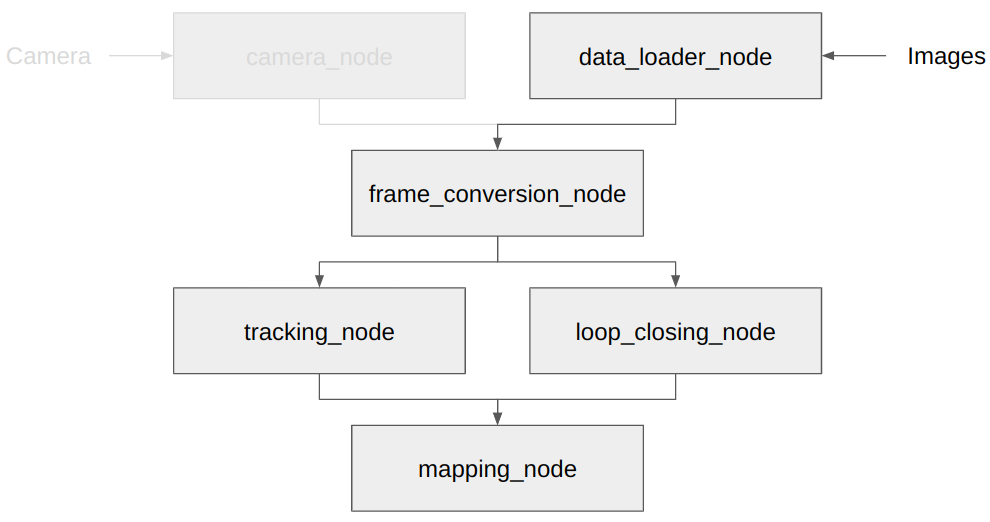
\includegraphics[width=0.5\textwidth]{img/pipeline.png}
    \caption{Visual SLAM pipeline}
    \label{fig:vslam_pipeline}
\end{figure}

Figure~\ref{fig:vslam_pipeline} shows the proposed visual SLAM pipeline with the components implemented as individual composable nodes. 
The role of each node is described as follows:
\begin{itemize}
  \item \hl{data\_loader\_node} takes in a list of images from a folder and convert them into OpenCV format and publish them sequentially.
  \item \hl{frame\_conversion\_node} 
  \item The text in the entries may be of any length.
\end{itemize}

* Use octree/octomap for managing map points 

\section{Appendix}

To ensure ROS2 is the right fit for the visual SLAM framework, we need to experiment with the modularity and the memory-sharing mechanism provided by it.
\href{https://github.com/ros-planning/navigation2}{Nav2} provides examples of creating action servers (e.g., planner and controller), each of which could have several plugins to accomplish various tasks.
The action servers are ROS2 nodes managed by their \href{https://github.com/ros2/demos/blob/humble/lifecycle/README.rst}{lifecycle manager} to activate or deactivate the nodes on demand.
The nodes are loaded as \href{https://docs.ros.org/en/humble/How-To-Guides/Launching-composable-nodes.html}{composable nodes} to allow for \href{https://docs.ros.org/en/humble/Tutorials/Demos/Intra-Process-Communication.html}{intra-communication} among the nodes.
Therefore, we could use action servers to represent the core components in the visual SLAM system and potentially use intra-process communication to reduce the overhead from unnecessary data copy between nodes.